
\section{Experimental Setup}

    To investigate the influence of the substrate geometry on static and dynamic observables, we place water droplets on PMMA cylinders with diameters $D \in \{ \num{2.19(2)},\, \num{3.99(2)},\, \num{5.15(4)},\, \num{10.2(2)} \} \, \text{mm}$, using a high-precision mechanical pipette by \textit{Sartorius} for $V \in [2.0, \, 20.0] \, \mu \text{l}$. 
    \begin{figure}[H]
        \centering
        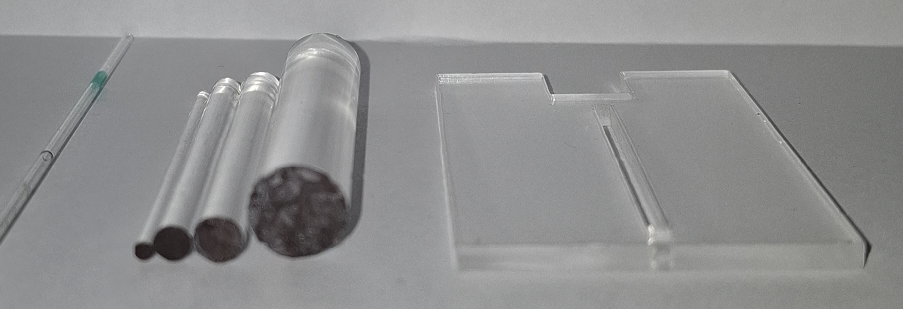
\includegraphics[width=\linewidth]{../Figs/photo_samples.PNG}
        \caption{Photo of PMMA samples and fixation plate. The cylinders' back sides are painted black to enhance contrast for measurements of $W$. }
        \label{fig:photo_samples}
    \end{figure}
    The cylinder is fixed on a movable platform using rubber bands and the oberservation is supported by a white backlight. All experimemts use twice-boilt tap water for the liquid droplets. 
    \begin{figure}[H]
        \centering
        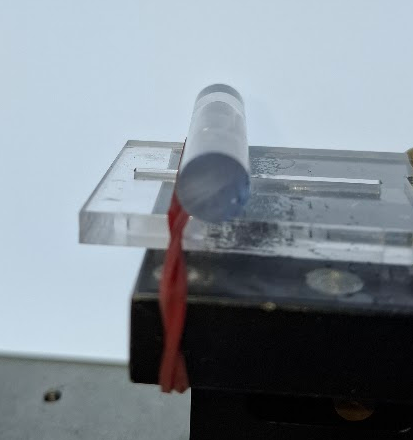
\includegraphics[width=0.41\linewidth]{../Figs/photo_measure_front.PNG}
        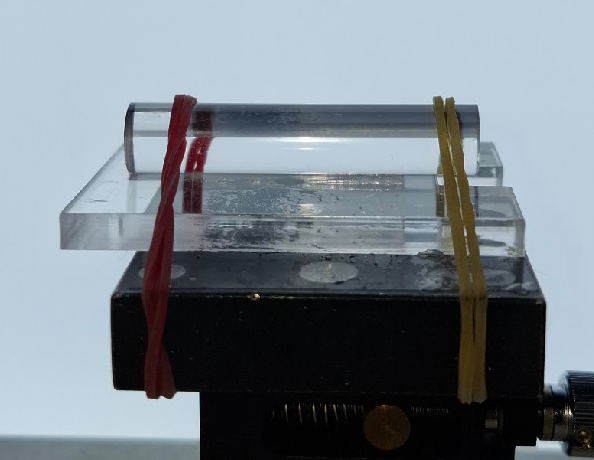
\includegraphics[width=0.56\linewidth]{../Figs/photo_measure_side.PNG}
        \caption{Photo from the camera perspective to measure $W(x)$ (left) and $L$ (right) on the \SI{10}{mm} cylinder fixed by rubber bands.}
        \label{fig:photo_measure}
    \end{figure}
    Finally, the photography is performed by the \textit{MEMRECAM GX-1} camera (C Mount Depth \SI{9}{mm}) with a narrow lens and fixed focus for upto 4x magnification. The high-speed camera is operated by the software \textit{MLink} and set to $50$ FPS and $250$ Shutter. The image format is set to $484$x$480$. To analyze the snapshot, the distances $L$ and $x$ are measured in pixels using the software \textit{ImageJ}. After each measurement, a pipe of known width is placed in the focus of the length to gauge the pixel size for a given magnification. 
    \begin{figure}[H]
        \centering
        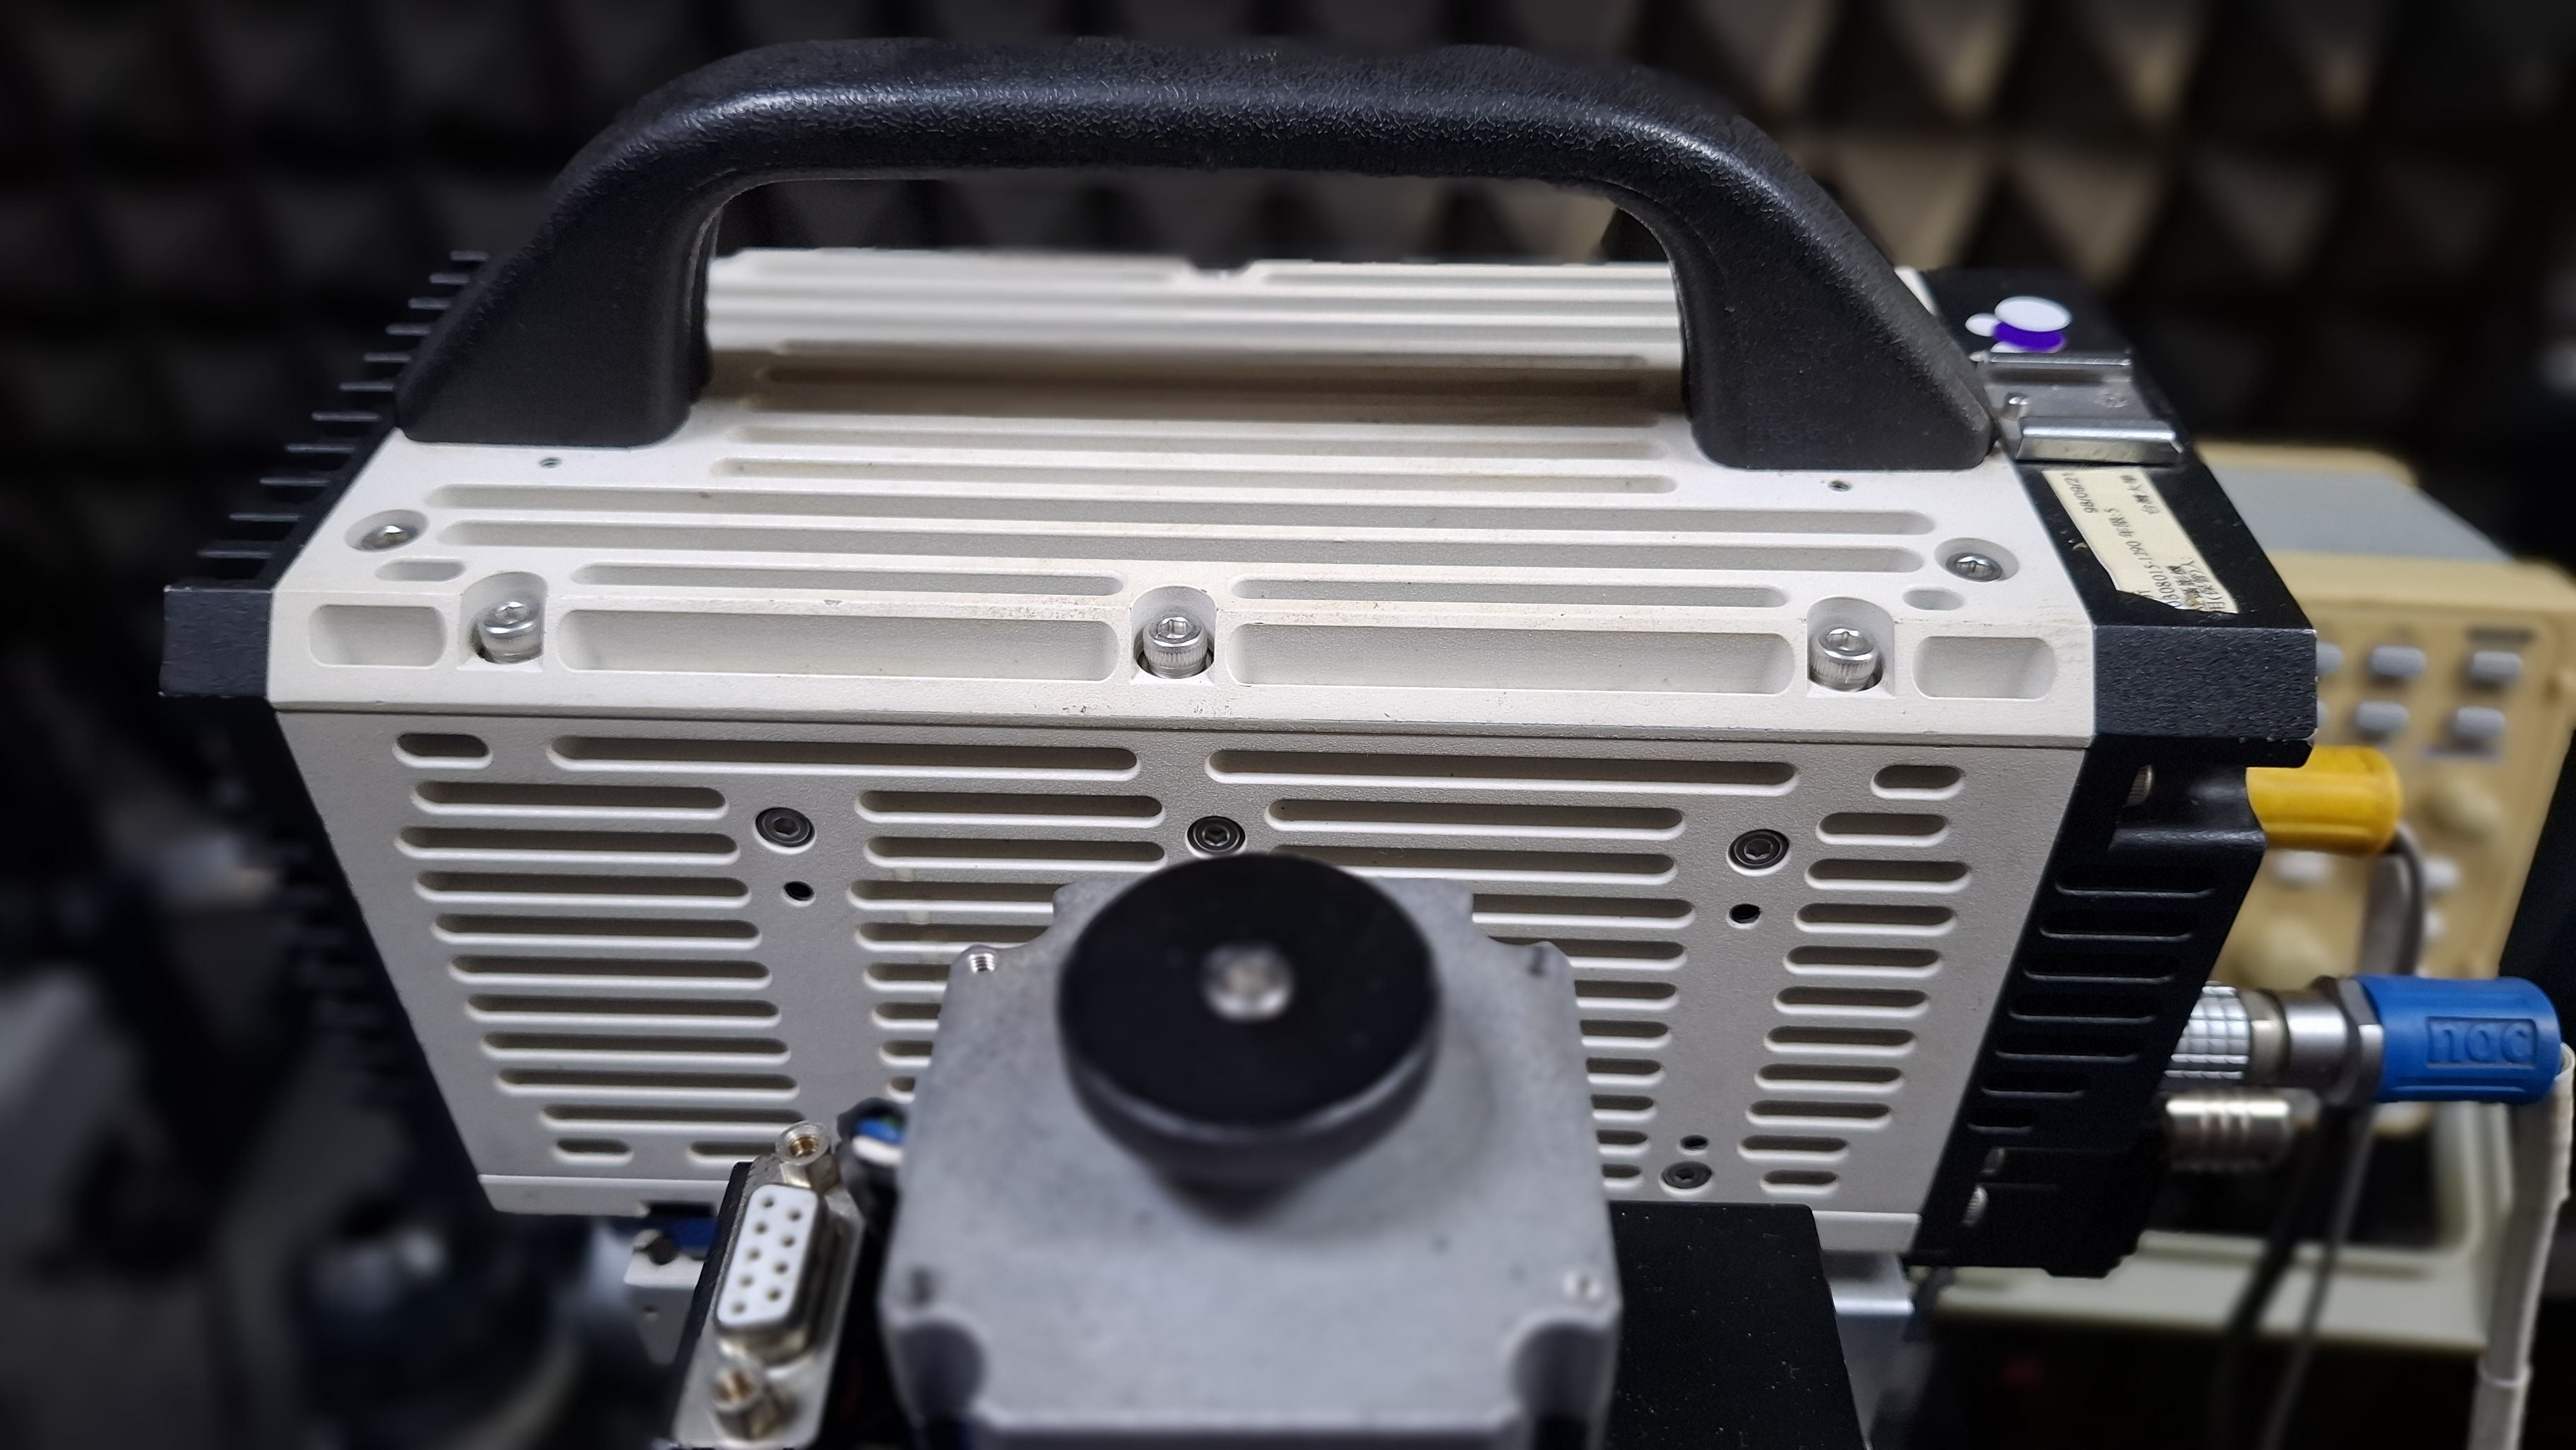
\includegraphics[width=0.9\linewidth]{../Figs/photo_camera_side.jpg}
        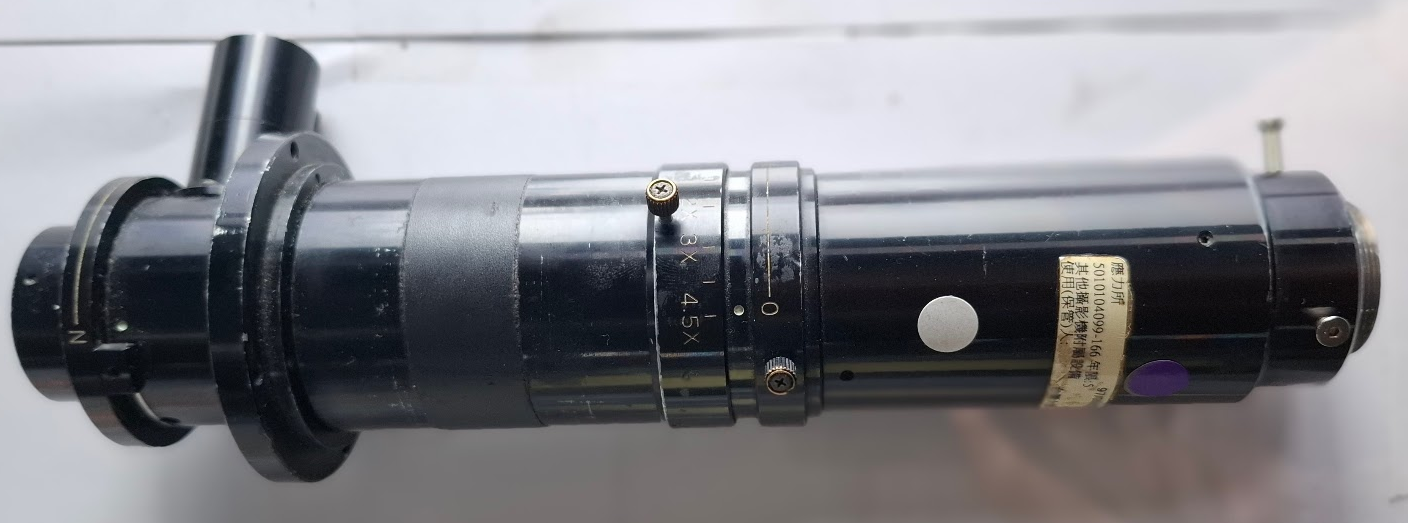
\includegraphics[width=0.9\linewidth]{../Figs/photo_lens.PNG}
        \caption{Photo of the high-speed camera (top) and the 4x magnification lens (bottom).}
        \label{fig:photo_camera}
    \end{figure}
    Between measurements, the sample cylinders are dried and cleaned from dust using \textit{Kimwipes$^{\text{TM}}$} for professional use. While the humidity in the laboratory cannot not be controlled accurately, the room temperature during experimental conduction lies between \SI{25}{\celsius} and \SI{29}{\celsius}. The backlight is not expected to contribute meaningfully to evaporation as it is not focused. 





\section{Measurement}

    For a measurement on a given cylinder $D$ for an array of droplet volumes $V$, the cylinder is cleaned using the wipes and fixed on the platform using rubber bands. Measurments of $W$ in the front position (\cref{fig:photo_measure}, left) are performed separately from measurements of $L$ in the side position (\cref{fig:photo_measure}, right) on different droplets. Therefore, no pair of $L$ and $W$ belong to the  same droplet. To make up for this lack in correspondance, each measurement is performed $4$ to $5$ times and averaged over. \\

    To place the droplets on the cylinder, one of two procedures is used:
    \begin{enumerate}
        \item The full volume of the droplet is placed on the cylinder as once, measured, cleaned off, and replaced by the next droplet volume of interest. This method is precise, but slow as the focus has to be readjusted each time. It is used for small cylinders $D < \SI{4}{mm}$.
        \item A \SI{2}{mm} droplet is placed, measured, and incremented to fit the next droplet volume of interest. The incrementation and measurement is repeated until the droplet becomes unstable and slides off the cylinder. This method is fast, but accumulates error due to the repeated manipulation of the droplet. It is used for large cylinders $D \geq \SI{4}{mm}$.
    \end{enumerate}
    It is assumed that the cylinder substrates do not \enquote{memorize} the exposure to previously applied droplets such that no additional waiting time is needed between measurements. \\

    \Cref{fig:example_2mm_2ul} shows an exemplary measurement on the \SI{2}{\milli\meter} cylinder, using the procedure (1). On PMMA, the experiment was repeated for droplet sizes \SI{2.2}{\milli\meter}, \SI{2.4}{\milli\meter}, \SI{2.6}{\milli\meter}, \SI{2.9}{\milli\meter}, and \SI{3.2}{\milli\meter}. Due to the limitations of the pipette, drop volumes below \SI{2}{\milli\meter} were inaccessible.
    \begin{figure}[H]
        \centering
        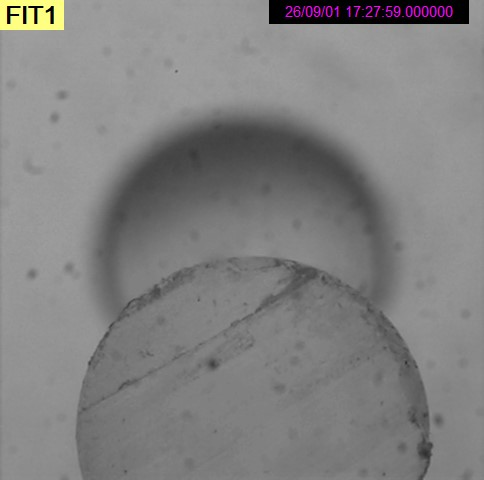
\includegraphics[width=0.32\linewidth]{../Figs/2_0ul_02mm_front-0.jpg}
        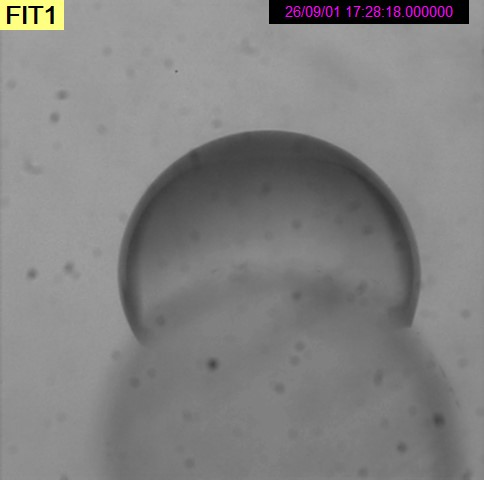
\includegraphics[width=0.32\linewidth]{../Figs/2_0ul_02mm_front-1.jpg}
        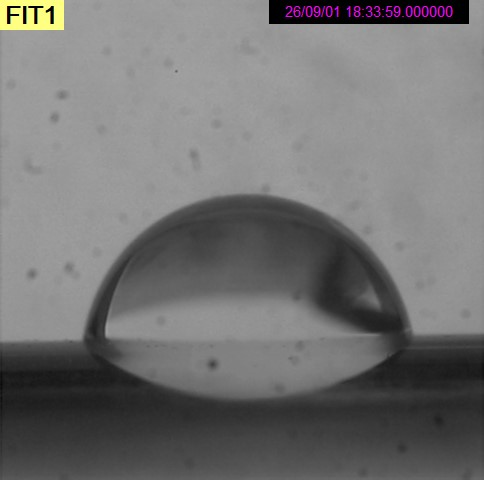
\includegraphics[width=0.32\linewidth]{../Figs/2_0ul_02mm_side-0.jpg}
        \caption{Measurement of a \SI{2}{\micro\liter} droplet on the \SI{2}{\milli\meter} cylinder from the front (left, middle) and side perspective (right). }
        \label{fig:example_2mm_2ul}
    \end{figure}
    On the \SI{4}{\milli\meter} cylinder (\cref{fig:example_4mm_6ul}), procedure (2) was used, incrementing a \SI{2}{\milli\meter} droplet to \SI{4}{\milli\meter}, \SI{6}{\milli\meter}, \SI{8}{\milli\meter}, \SI{10}{\milli\meter}, and \SI{12}{\milli\meter}. The \SI{12}{\milli\meter} measurement, however, showed repeated instability and therefore cannot be analyzed. 
    \begin{figure}[H]
        \centering
        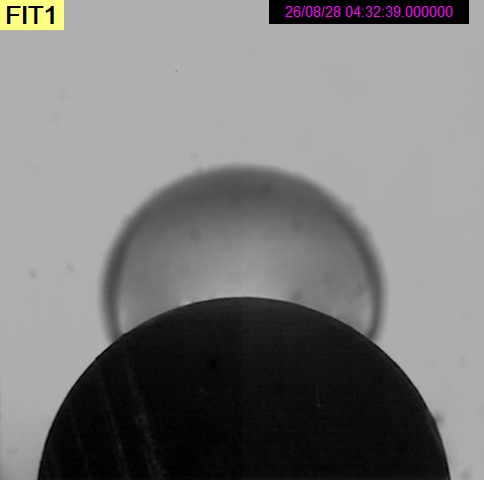
\includegraphics[width=0.49\linewidth]{../Figs/06ul_04mm_front-3.jpg}
        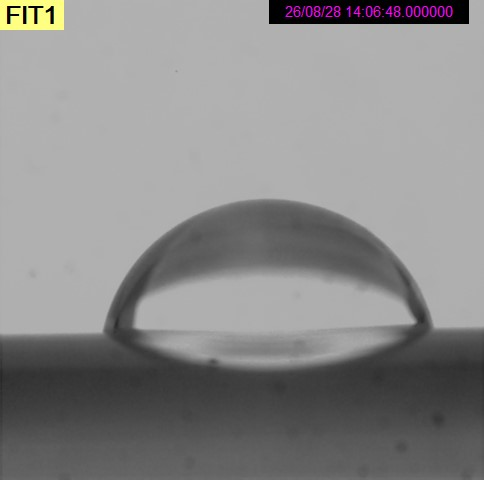
\includegraphics[width=0.49\linewidth]{../Figs/06ul_04mm_side-2.jpg}
        \caption{Measurement of a \SI{6}{\micro\liter} droplet on the \SI{4}{\milli\meter} cylinder from the front (left) and side perspective (right). }
        \label{fig:example_4mm_6ul}
    \end{figure}
    Similarly, on the \SI{10}{\milli\meter} cylinder (\cref{fig:example_10mm_16ul}), procedure (2) was used, incrementing a \SI{2}{\milli\meter} droplet to \SI{4}{\milli\meter}, \SI{8}{\milli\meter}, \SI{12}{\milli\meter}, \SI{16}{\milli\meter}, \SI{20}{\milli\meter}, and \SI{30}{\milli\meter}. The \SI{30}{\milli\meter}, however, showed repeated instability and therefore cannot be analyzed. 
    \begin{figure}[H]
        \centering
        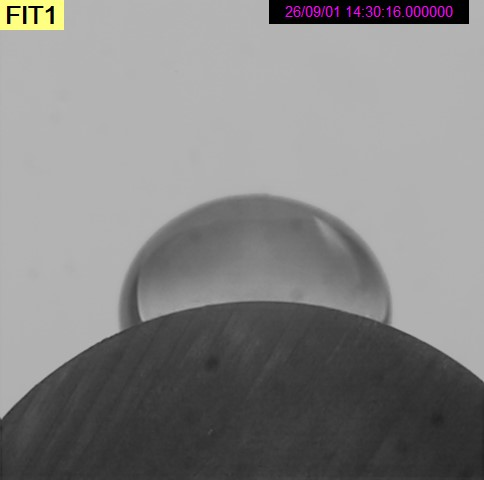
\includegraphics[width=0.49\linewidth]{../Figs/16ul_10mm_front-1.jpg}
        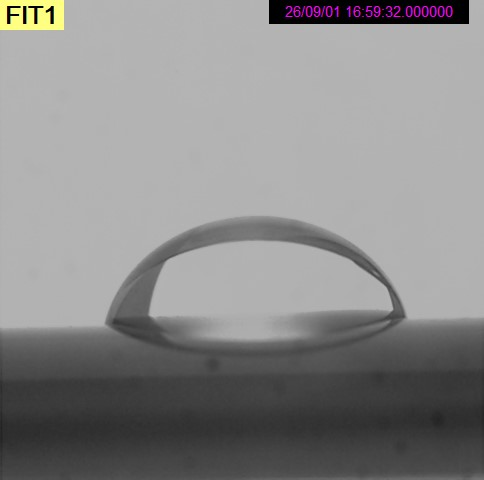
\includegraphics[width=0.49\linewidth]{../Figs/16ul_10mm_side-5.jpg}
        \caption{Measurement of a \SI{16}{\micro\liter} droplet on the \SI{10}{\milli\meter} cylinder from the front (left) and side perspective (right). }
        \label{fig:example_10mm_16ul}
    \end{figure}
    Note that due to the short focus length of the camera, is was not always possible to focus the droplet's silhouette and the cylinder at the same time. In these cases, the focus on the cylinder is preferred as it showed to be more precise and reliable than focussing the droplets individually. \\

    We assume a relative uncertainty of \SI{5}{\percent} for all lenghts measured in the images ($L$, $x$, gauge pipe) due to the limitations of the camera focus and image quality. Moreover, this uncertainty is meant to compensate for small deviations in droplet volume and induced vibrations during droplet placement. Generally speaking, there are countless possible sources of systematic error such as changes in room temperature and humidity, pollution of the sample and liquid, inaccurate camera placement, and evaporation. We nethertheless believe that the dominant source of uncertainty is caused by the droplet placement and sample impurity. 









\section{Results}



\section{Conclusion}



    \begin{figure}[H]
        \centering
        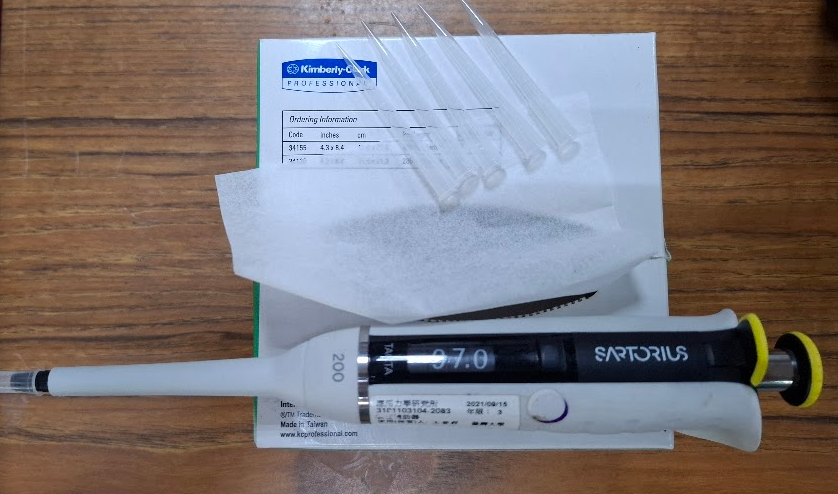
\includegraphics[width=\linewidth]{../Figs/photo_pipette.PNG}
        \caption{Photo of the \SI{2}{\micro\liter} to \SI{20}{\micro\liter} pipette with \textit{KG1213-L} Low Binding Pipette Tips by \textit{Kirgen}. }
        \label{fig:photo_pipette}
    \end{figure}
